\section{Overlapping Data Transfers}
\label{sec-async}

In this section, we talk about the details of streaming data transfers. Then we go on and talk about how we implement the streaming transfers in Gluon~\cite{dathathri2018gluon}. We then discuss about the implementation and the challenges that we faced during the implementation. 

\subsection{Streaming Data Transfers}

A stream in CUDA is a sequence of operations that execute on the device in the order in which they are issued by the host code. While operations within a stream are guaranteed to execute in the prescribed order, operations in different streams can be interleaved and, when possible, they can even run concurrently. All device operations (kernels and data transfers) in CUDA run in a stream. When no stream is specified, the default stream (also called the ``null stream") is used. The default stream is different from other streams since it synchronizes with 
other kernel or data transfer streams on the device: no operation in the default stream will begin until all previously issued operations in any stream on the device have completed, and an operation in the default stream must complete before any other operation (in any stream on the device) will begin.

\begin{figure}
\centering
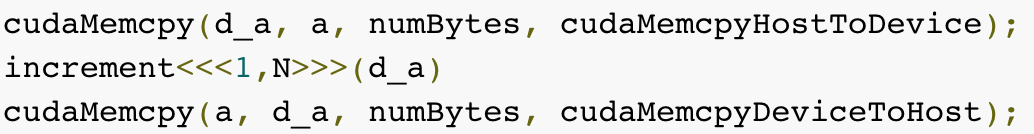
\includegraphics[width=0.49\textwidth]{async-serial.png}
\mycaption{}{This figure shows an algorithm for serially performing communication and computation. }
\label{fig-async-serial}
%\vspace{-20pt}
\end{figure}

\begin{figure}
\centering
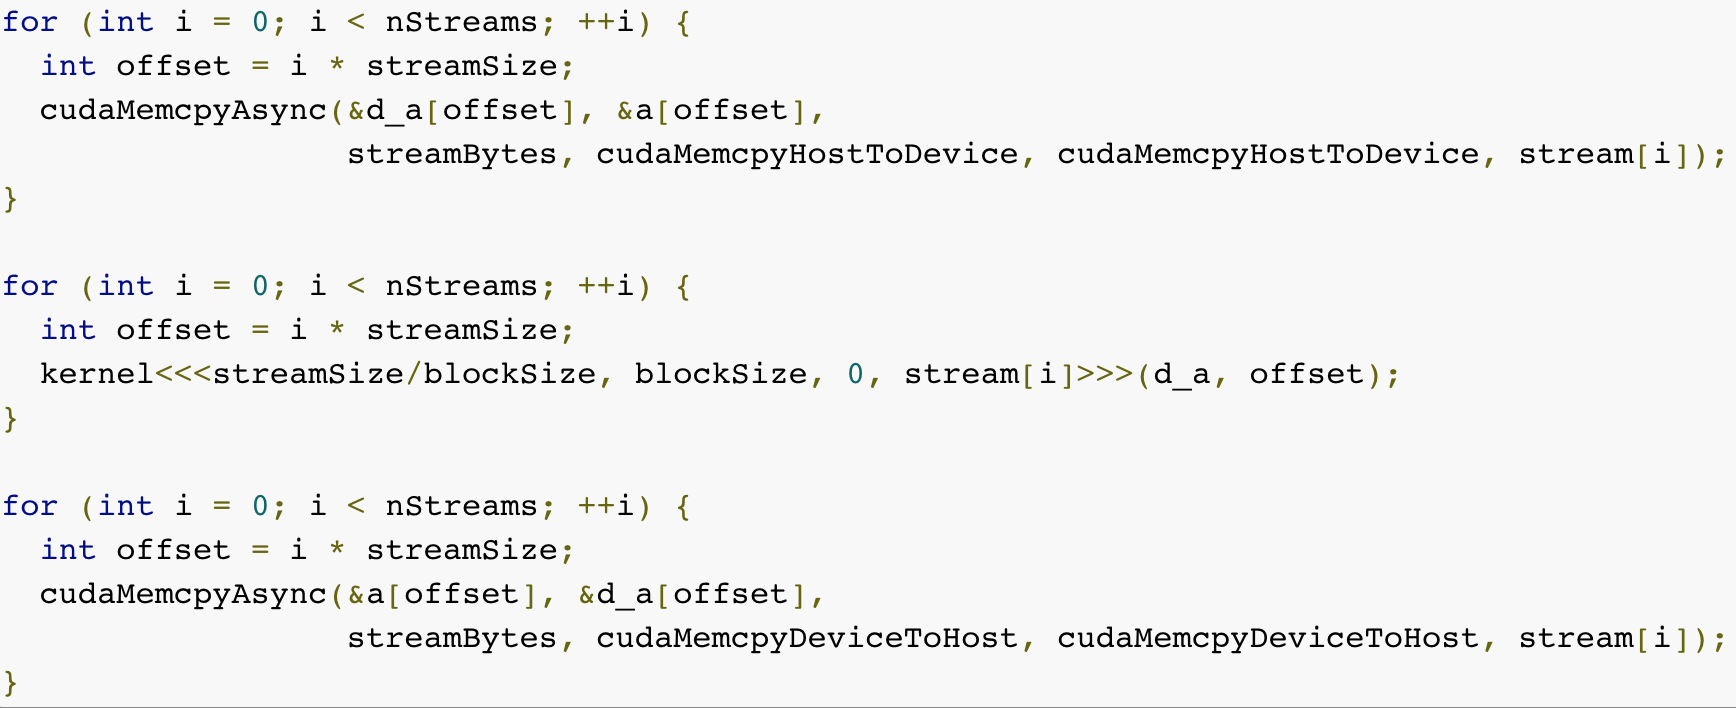
\includegraphics[width=0.49\textwidth]{async-parallel.png}
\mycaption{}{This figure shows an algorithm for overlapping communication and computation. }
\label{fig-async-parallel}
%\vspace{-20pt}
\end{figure}

The main goal behind streaming data transfers is 
overlapping kernel execution along with data transfers. 
For this to be successful, the kernel execution and the data transfer should both occur in different, non-default streams. Also, the host memory that is involved in streaming data transfers should be pinned memory, if we want to achieve maximum performance. Figure ~\ref{fig-async-serial} shows the algorithm that uses default stream, which does not overlap computation with communication, whereas Figure~\ref{fig-async-parallel} shows the same algorithm that overlaps computation with communication using non-default streams. Note that both the algorithms provide current results, but the performance varies significantly. 

\begin{figure}
\centering
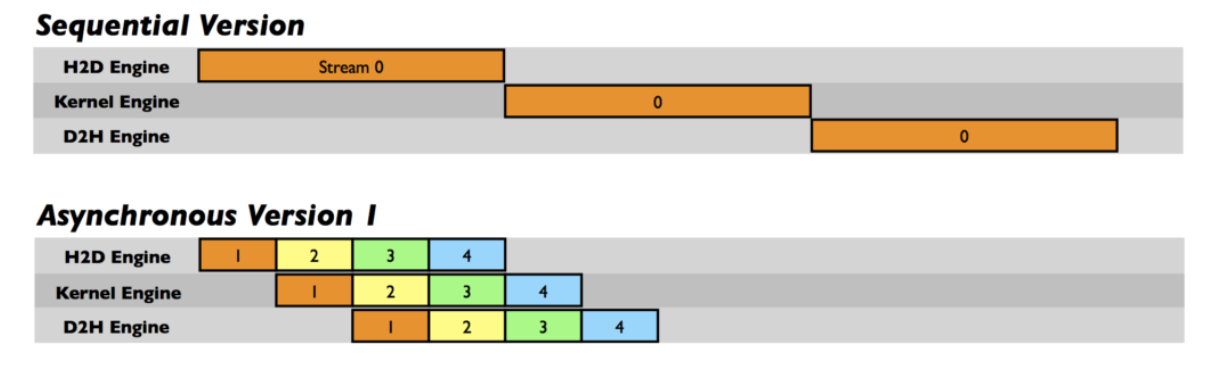
\includegraphics[width=0.49\textwidth]{async-perf.png}
\mycaption{Streaming data performance}{This figure shows the difference in performance between serial and overlapping communication with computation }
\label{fig-async-perf}
%\vspace{-20pt}
\end{figure}

Figure~\ref{fig-async-perf} shows the execution timelines for the sequential algorithm versus the asynchronous algorithm that overlaps computation with communication. As we can see from this figure, the end-to-end latency of the sequential version is roughly 2X compared to the asynchronous version. 

\subsection{Asynchronous Transfers in Gluon}

In the Gluon substrate, during the communication of graph data from a source node (or master node) to a destination node (or mirror node), the following steps take place, in a sequential order:
\begin{enumerate}
\item The offset and the bitset for the updated nodes are computed at GPU of the source host.
\item The offset, the bitset and the updated node label data are copied from GPU to CPU and serialized into a CPU buffer.
\item The serialized CPU buffer is transferred to the destination host.
\item The arrived CPU buffer at the destination is deserialized and copied to the GPU.
\item During the copy, proper locations are computed and the copied buffer is scattered across them.
\end{enumerate}

We modified these synchronization phase in order to asynchronosly process and overlap the computations.
First, we overlapped the computation of the step 1 with the data copy from GPU to CPU of the step 2.
Second, we overlapped the data copy from CPU to GPU of the step 4 with the computation on the copied data of the step 5
using asynchronous streaming data transfers.

\subsection{Discussion}

The suggested objective of this project is overlapping among multiple data transfers with multiple GPU streams.
Therefore, the first challenge that we faced was to find the exact position where it is possible to asynchronously 
transfer data in the large code base.
To do this, we chose one specific target application, bfs\_push of lonstardist.
We finally found locations where we can apply the asynchronous data transfers on the synchronization parts.


For this project, we focused on memory-memory computation overlapping; this is just our prototype implementations
of overlapping data transfers using asynchronous memory transfers.
We strongly believe that it would be possible to overlap other parts such as
overlapping between BFS computations and data transfers.


The second challenge was regarding the use of pinned memory for the asynchronous transfers. 
Pinned memory could be exploited efficiently for the streaming data transer.
Instead of using page-able memory managed by kernel, specific memory ranges are fixed and used for data transfer.
One limitation of pinned memory is that pinned memory cannot be reallocated or resized once it is allocated.
This is critical since we cannot efficiently use pinned memory for sparse data, which could frequently resize its size.
It is hard to expect the size of the sparse data.
Especially, our target application, round based bfs\_push, changes its frontier node labels and 
correspondig auxiliary data for each round.
Therefore, we could not directly use the pinned memory feature and hence, we believe that it won't 
lead to maximum performance improvements from the asynchronous data transfers.
There needs to be a comprehensive change in the Gluon code to apply pinned memory, which might lead to better performance.


